%==============================================================================
%  Architecture and Preprocessing Choices under Dataset Shift in Single-Channel
%  EEG Sleep Staging: A Controlled Evaluation on Sleep-EDF and SHHS1
%
%  English manuscript. Journal-neutral single-column preprint format.
%  Build:  pdflatex -> bibtex -> pdflatex -> pdflatex
%==============================================================================
\documentclass[11pt,a4paper]{article}

\usepackage[T1]{fontenc}
\usepackage[utf8]{inputenc}
\usepackage[english]{babel}
\usepackage{newtxtext,newtxmath}   % Times-like text + math (journal convention)
\usepackage{microtype}
\usepackage{geometry}
\usepackage{amsmath}
\usepackage{graphicx}
\usepackage{booktabs}
\usepackage{tabularx}
\usepackage{array}
\usepackage{multirow}
\usepackage{caption}
\DeclareCaptionType{suppfig}[Supplementary Figure]{}
\usepackage{subcaption}
\usepackage[section]{placeins}
\usepackage{xcolor}
\usepackage{enumitem}
\usepackage{xurl}
\usepackage{xr-hyper}
\usepackage{hyperref}
\externaldocument[SM-]{supplement}[supplement.pdf]
\usepackage{fancyhdr}
\usepackage{authblk}               % structured author / affiliation block
\usepackage{titlesec}
\usepackage{abstract}

\geometry{top=2.4cm,bottom=2.4cm,left=2.3cm,right=2.3cm}
\setlength{\parindent}{1.1em}
\setlength{\parskip}{0.2em}
\setlist{nosep,leftmargin=1.6em}
\captionsetup{font=small,labelfont=bf,labelsep=period}
\renewcommand{\arraystretch}{1.15}
\newcolumntype{Y}{>{\raggedright\arraybackslash}X}
\newcolumntype{C}[1]{>{\centering\arraybackslash}p{#1}}

% ---- section headings: journal-style, not oversized -------------------------
\titleformat{\section}{\normalfont\large\bfseries}{\thesection.}{0.6em}{}
\titleformat{\subsection}{\normalfont\normalsize\bfseries}{\thesubsection.}{0.6em}{}
\titleformat{\subsubsection}{\normalfont\normalsize\itshape}{\thesubsubsection.}{0.6em}{}
\titlespacing*{\section}{0pt}{1.5ex plus .3ex}{0.8ex}
\titlespacing*{\subsection}{0pt}{1.2ex plus .3ex}{0.6ex}

% ---- author block formatting (authblk) --------------------------------------
\renewcommand\Authfont{\normalsize}
\renewcommand\Affilfont{\small\itshape}
\setlength{\affilsep}{0.7em}
\renewcommand\Authands{, }         % no "and" before the last author
\renewcommand\Authsep{, }

% ---- abstract block ---------------------------------------------------------
\renewcommand{\abstractnamefont}{\normalfont\bfseries}
\renewcommand{\abstracttextfont}{\normalfont\small}
\setlength{\absleftindent}{0.6cm}
\setlength{\absrightindent}{0.6cm}

\definecolor{linkblue}{RGB}{18,82,148}
\hypersetup{
  colorlinks=true,
  linkcolor=linkblue,
  citecolor=linkblue,
  urlcolor=linkblue,
  pdftitle={Architecture and Preprocessing Choices under Dataset Shift in Single-Channel EEG Sleep Staging: A Controlled Evaluation on Sleep-EDF and SHHS1},
  pdfauthor={Ngo Nhat Quan; Pham Thai Son},
  pdfkeywords={sleep staging; single-channel EEG; temporal convolutional network; preprocessing; domain shift; paired evaluation}
}

\pagestyle{fancy}
\fancyhf{}
\fancyhead[L]{\small\itshape Ngo and Pham}
\fancyhead[R]{\small\itshape Pipeline choices under sleep-staging dataset shift}
\fancyfoot[C]{\thepage}
\setlength{\headheight}{14pt}
\renewcommand{\headrulewidth}{0.4pt}

\newcommand{\mf}{\ensuremath{\mathrm{macro\text{-}F1}}}
\newcommand{\ci}{\ensuremath{\mathrm{CI}_{95\%}}}
\newcommand{\dsign}{\ensuremath{\Delta_{\mathrm{sign}}}}

%==============================================================================
\begin{document}

%------------------------------------------------------------------ front matter
\title{\bfseries\LARGE Architecture and Preprocessing Choices under Dataset Shift\\[0.15em]
in Single-Channel EEG Sleep Staging:\\[0.15em]
A Controlled Evaluation on Sleep-EDF and SHHS1}

\author[1,$\ast$]{Ngo Nhat Quan}
\author[1]{Pham Thai Son}
\affil[1]{Faculty of Information Systems, University of Information Technology,\protect\\
Vietnam National University Ho Chi Minh City, Ho Chi Minh City, Viet Nam}

\date{}

\maketitle
\thispagestyle{empty}

\vspace{-1.0em}
\begin{center}
\small
Ngo Nhat Quan: \texttt{23521258@gm.uit.edu.vn} $^{\ast}$(Corresponding author) \\[0.2em]
Pham Thai Son: \texttt{23521361@gm.uit.edu.vn}
\end{center}

\vspace{0.4em}
\begin{center}\rule{0.9\textwidth}{0.4pt}\end{center}
\vspace{-0.2em}

\begin{abstract}
\noindent
\textbf{Background.} Improvements in sleep staging on one dataset may not carry over to another.
We examined how model and preprocessing choices affect accuracy, computational cost and cross-cohort errors.

\noindent
\textbf{Methods.} Six configurations were compared on 78 Sleep-EDF subjects using shared 10-fold
partitions. Comparisons covered sequence-model and training-recipe replacement, a bundled encoder/context
replacement, and preprocessing. Paired subject bootstrap and Wilcoxon--Holm analysis assessed uncertainty.
Transfer used 180 locked SHHS1 participants without weight updates. Record-wise normalisation used each
complete unlabelled target recording and was therefore transductive.

\noindent
\textbf{Results.} The fixed-scale ResNet-1D--TCN configuration (E3) reached Sleep-EDF \mf\ 0.7904
in the primary campaign, exceeding its record-wise-normalised counterpart (E6) by 0.0213
(\ci\ $[0.0122,0.0307]$; Holm $p=0.0012$). A second seed preserved the direction but not Holm
significance. E3 delivered a $3.76\times$ forward-pass speed-up over the CNN--BiLSTM control,
with $4.37\times$ as many parameters and 28.4\% more peak memory. On SHHS1, it improved subject-mean
\mf\ over the control by 0.0412 (\ci\ $[0.0314,0.0512]$). Yet both pipelines misclassified
over 72\% of N3 epochs as N2; N3 recall was 0.2610 for the control, 0.2582 for E3 and 0.2005 for E6.

\noindent
\textbf{Conclusions.} The evaluated pipeline combined faster computation with improved aggregate
cross-cohort performance and revealed a shared cross-cohort N3 under-detection pattern across both model
families. Preprocessing choices and stage-specific errors are consequential alongside model design when
assessing cross-cohort use.
\end{abstract}

\vspace{0.3em}
\noindent\textbf{Keywords:} sleep staging; single-channel EEG; temporal convolutional network;
preprocessing; domain shift; paired evaluation.

\vspace{0.3em}
\begin{center}\rule{0.9\textwidth}{0.4pt}\end{center}

%==============================================================================
\section{Introduction}

Sleep staging assigns one of five labels---W, N1, N2, N3 and REM---to every 30\,s epoch of a
polysomnographic recording. Manual scoring is slow, requires trained expertise, and retains
irreducible disagreement between scorers; in the inter-scorer reliability programme of the American
Academy of Sleep Medicine, N1 shows the lowest agreement of all stages~\cite{rosenberg2013aasm}. An
automated system therefore has to be judged not by overall accuracy alone, which is dominated by the
most frequent stages, but by class-balanced metrics, by stability across individuals, and by its
behaviour when the recording device, montage or population changes.

Progress in this field is difficult to read from published tables. Studies differ simultaneously in
dataset version, subject partitioning, wake-trimming policy, filtering, normalisation, sequence length
and model-selection rule, so a reported improvement cannot be attributed to the architecture that the
paper nominally proposes. For practical development, the relevant questions are which pipeline choices
improve prediction, what they cost computationally, and whether their benefits persist on another cohort.
Answering these questions requires shared evaluation partitions and an explicit account of what changes
between configurations, including their training procedures.

We take ZleepAnlystNet~\cite{jadhav2024zleepanlystnet}, a two-stage single-channel model that couples a
bank of class-specific convolutional encoders to a BiLSTM, as an internal control. E1 replaces the
BiLSTM configuration with a temporal convolutional network (TCN)~\cite{bai2018tcn}, reusing the encoder
and cached features but changing the sequence-model training recipe. E2 replaces E1's 75-dimensional
current/previous/next (C/P/N) feature-context package with a 128-dimensional current-epoch residual
encoder~\cite{he2016resnet}, also changing encoder training and selection. These are comparisons of
specified configurations, not isolated architectural effects. Preprocessing contrasts then examine
filtering and amplitude handling within the same ResNet-1D--TCN model and training configuration.

The study addresses three questions. (i) What predictive and computational benefits do the evaluated
sequence-model and encoder/context replacements provide under shared subject-wise partitions?
(ii) Which pipeline choices retain their benefits when transferred without weight updates to a separate
cohort with a different EEG derivation? (iii) Which class confusions recur across model families, and
how are they distributed between reference-label boundaries and stable sleep regions?

Our contributions are the following.

\begin{enumerate}[label=(\arabic*)]
\item A 10-fold subject-wise evaluation that compares six configurations on shared partitions,
documents their model and training differences, and pairs aggregate effects with subject-level inference.
\item A locked cross-cohort evaluation on 180 SHHS Visit-1 participants, showing that the ranking and
magnitude of design choices can differ between internal validation and cross-cohort use.
\item A class- and confusion-channel analysis revealing a shared cross-cohort N3 under-detection pattern
across the 15-CNN--BiLSTM control and ResNet-1D--TCN, while over-detection of REM from N2 is a second
prominent E3 error channel. The evaluated record-wise normalisation pipeline does not change this pattern.
\item A quantified operational trade-off: the implemented ResNet-1D--TCN pipeline reduces measured
forward latency and training-and-validation wall-clock time relative to the 15-branch CNN--BiLSTM
control, while increasing parameter count and peak memory. These operational gains are distinguished
from predictive differences within and across cohorts.
\end{enumerate}

%==============================================================================
\section{Related work}

DeepSleepNet combined a dual-branch CNN with a BiLSTM to capture epoch morphology and temporal
dependence~\cite{supratak2017deepsleepnet}. AttnSleep introduced attention over multi-resolution
features~\cite{eldele2021attnsleep}, and SleepTransformer applied self-attention with explicit
uncertainty quantification~\cite{phan2022sleeptransformer}. Together these establish that sequential
context matters substantially. They also illustrate the comparability problem: differences in dataset
version, subject split and preprocessing between these works are large enough that cross-table
comparison cannot substitute for an ablation carried out inside one protocol, a point emphasised in
recent reviews of the field~\cite{phan2022review}.

Single-channel systems also span materially different input representations. SleepInceptionNet
systematically compared raw, spectral and time--frequency inputs and selected a continuous-wavelet,
central-channel Inception model that scores one epoch at a time~\cite{haghayegh2023sleepinceptionnet}.
That study reinforces two points relevant here: a single EEG channel can support five-stage scoring, and
preprocessing choice is part of the model definition rather than a neutral implementation detail.

Cross-dataset sleep staging is already an active methodological problem. For example, He et
al.~\cite{he2023crossscenario} trained a domain-adaptation network across Sleep-EDF, SHHS1 and the
PhysioNet Challenge data. ADAST instead uses domain-specific attention, adversarial alignment and
iterative pseudo-label self-training on unlabelled target data~\cite{eldele2023adast}. These approaches
adapt model representations or decision functions using the target domain; our label-free E6 condition
only estimates recording-level normalisation statistics, with no learned target-domain or weight adaptation.
Van Der Donckt et al.~\cite{vdd2023traditional} further showed that increasingly complex deep
architectures need not outperform a carefully designed conventional pipeline under a matched protocol.
Our contribution is a joint assessment of pipeline substitutions, preprocessing, computational cost
and cross-cohort error structure. The paired comparisons quantify benefits within a common protocol;
the cross-model analysis tests whether an aggregate transfer gain also addresses the dominant stage-specific
failure. Neither question is answered by comparing scores from unrelated benchmark tables.

Sleep-EDF Expanded is the standard public benchmark for single-channel
EEG~\cite{kemp2000sleepEDF,physionetSleepEDF}. The Sleep Heart Health Study (SHHS) is a large
multi-centre cohort assembled to study sleep-disordered breathing and cardiovascular
risk~\cite{quan1997shhs}, distributed through the National Sleep Research Resource
(NSRR)~\cite{zhang2018nsrr}. The two differ in age, comorbidity, recording hardware, montage and label
distribution. SHHS therefore tests a form of cohort change not represented by a held-out split of
Sleep-EDF. We use it to assess cross-cohort robustness, without equating retrospective transfer testing
with clinical deployment validation.

Two further strands of work inform the interpretation. Slow oscillations have a spatially varying
amplitude and propagate across the cortex~\cite{massimini2004travelling}, while deep-sleep scoring uses
amplitude criteria~\cite{rechtschaffen1968,berry2017aasm}. A recent SHHS analysis examined how those
criteria relate to age- and sex-associated differences in N3 scoring~\cite{davidson2025n3}. Such work
provides context for transfer between derivations and populations, rather than a mechanism established
by the present experiment. Differences in class prevalence can also affect predictions; prior correction
and probability calibration address related but distinct problems~\cite{saerens2002adjusting,guo2017calibration}.
We therefore examine class-wise errors and label proportions without treating marginal prediction
counts as a calibration measure.

%==============================================================================
\section{Materials and methods}

\subsection{Data and labels}

The Sleep Cassette subset of Sleep-EDF Expanded comprises 153 recordings from 78 subjects; we use the
Fpz--Cz derivation at 100\,Hz with 30\,s epochs (3{,}000 samples per epoch). Annotations are mapped to
W, N1, N2, N3 and REM, merging the original stages 3 and 4 into N3; Movement and Unknown epochs retain their temporal position but are excluded from
the loss and from all metrics. After windowing, 195{,}767 epochs remain, of which 195{,}469 are scored
and 298 are Movement/Unknown.

An evaluation window is applied identically to both cohorts. It is anchored on the first and last true
sleep epoch (any of N1, N2, N3, REM) and extended by 30\,min of wake on each side, i.e.\ 60 epochs per
side. This policy is stated explicitly because it strongly affects the wake fraction and hence every
aggregate metric, and because it is one of the principal reasons published numbers are not directly
comparable. It is a benchmark window, not a deployable inference rule, since its anchors use ground-truth
labels.

The SHHS Visit-1 selection used the metadata quality field \texttt{overall\_shhs1}, admitting values
3--7. Eligible participant identifiers were ranked deterministically by SHA-256 with selection seed 42,
then independently ranked for role assignment: 5 adaptation, 15 validation, 180 test and 20 reserve
participants. No reserve replacements were required. The 180-person test sample was locked before
prediction review; the adaptation and validation participants were not used to update model weights.
The EEG channel is C4--A1 at 125\,Hz, resampled to 100\,Hz with a polyphase anti-aliasing
filter (up 4, down 5, Kaiser window $\beta = 5.0$) applied to the continuous signal before epoching.
SHHS labels are mapped $0\rightarrow$W, $1\rightarrow$N1, $2\rightarrow$N2, $\{3,4\}\rightarrow$N3,
$5\rightarrow$REM, $\{6,9\}\rightarrow$excluded. Table~\ref{tab:class-distribution} reports both label
distributions.

\begin{table}[t]
\centering
\caption{Scored-label distribution in the two evaluation samples.}
\label{tab:class-distribution}
\small
\begin{tabular}{lrr|rrr}
\toprule
\textbf{Stage} & \multicolumn{2}{c|}{\textbf{Sleep-EDF}} & \multicolumn{3}{c}{\textbf{SHHS1 test}} \\
 & \textbf{Epochs} & \textbf{Share} & \textbf{Epochs} & \textbf{Share} & \textbf{Ratio to EDF} \\
\midrule
W   & 65{,}941 & 33.73\% & 36{,}983 & 21.88\% & 0.65 \\
N1  & 21{,}522 & 11.01\% & 7{,}002  & 4.14\%  & 0.38 \\
N2  & 69{,}132 & 35.37\% & 76{,}287 & 45.14\% & 1.28 \\
N3  & 13{,}039 & 6.67\%  & 22{,}806 & 13.49\% & 2.02 \\
REM & 25{,}835 & 13.22\% & 25{,}934 & 15.34\% & 1.16 \\
\midrule
\textbf{Total scored} & \textbf{195{,}469} & \textbf{100\%} & \textbf{169{,}012} & \textbf{100\%} & \\
\bottomrule
\end{tabular}
\end{table}

The prior shift between cohorts is substantial: total variation distance $0.187$,
$D_{\mathrm{KL}}(\text{EDF} \,\|\, \text{SHHS}) = 0.101$ nats. SHHS1 contains proportionally
$2.02\times$ as much N3 and $0.38\times$ as much N1. We report the per-class ratios in
Table~\ref{tab:class-distribution} because Section~\ref{sec:gap} uses their \emph{direction} as evidence.

\subsection{Preprocessing conditions}

To evaluate the individual and joint impacts of architectural design and preprocessing choices, we
propose an end-to-end processing pipeline, as illustrated in Figure~\ref{fig:pipeline}. The signal is
first calibrated and processed continuous-wise to preserve amplitude relationships, after which a
1D-ResNet epoch encoder and a TCN sequence model extract local and temporal characteristics,
respectively.

\begin{figure}[htbp]
    \centering
    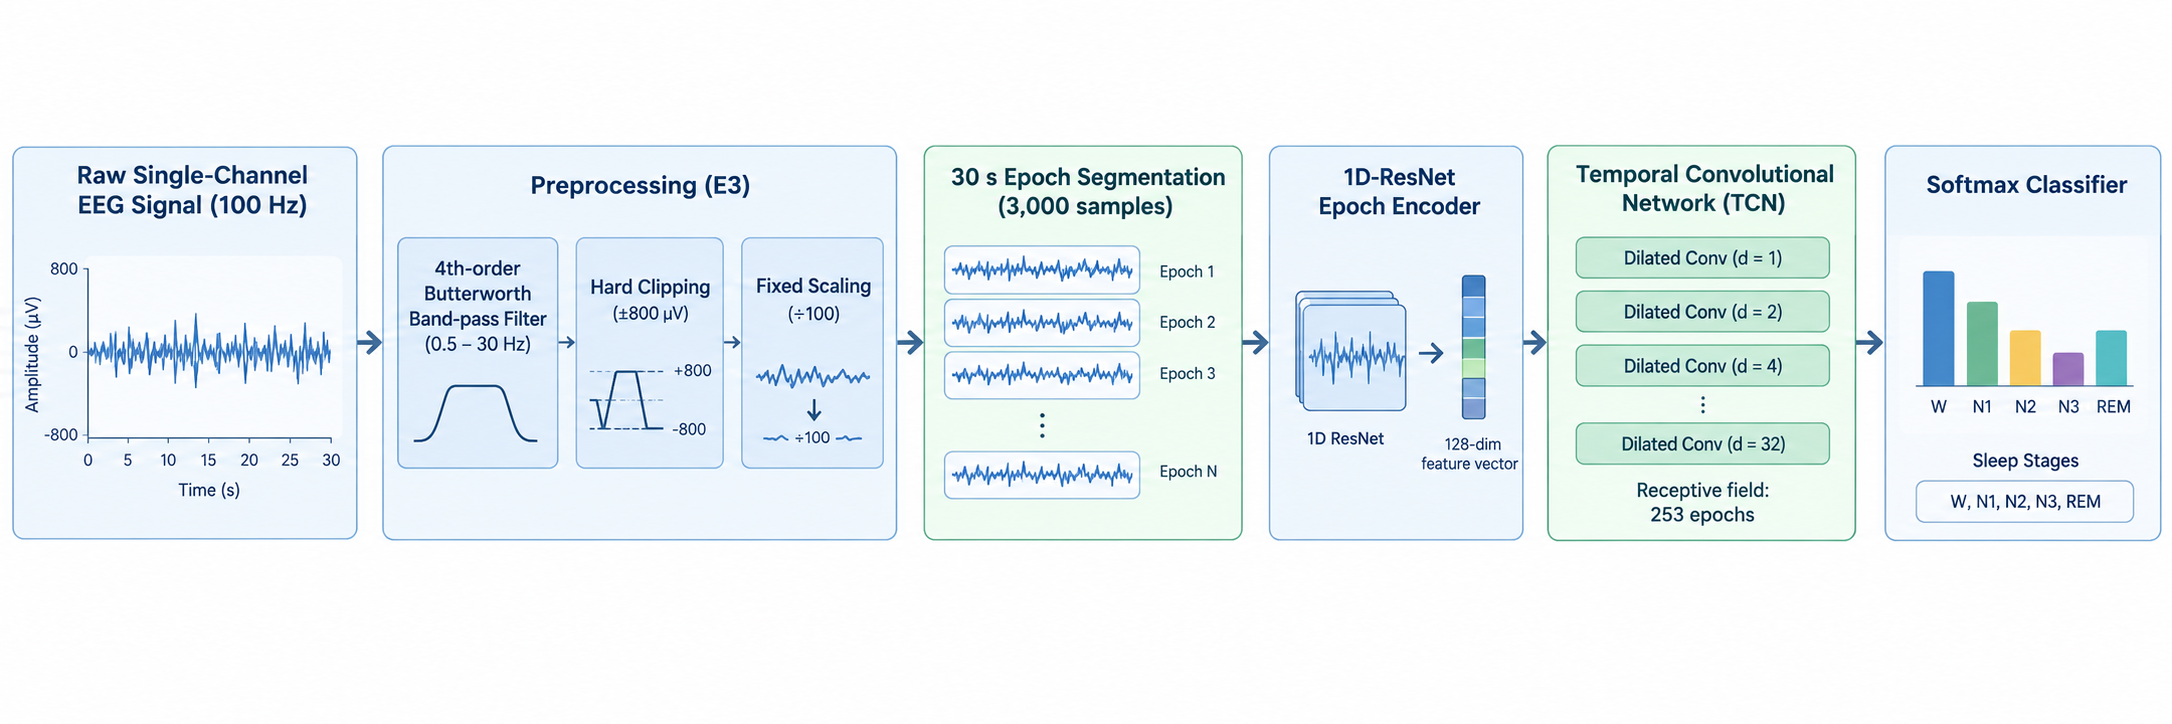
\includegraphics[width=0.9\textwidth]{./figures/gate8_pipeline_overview_en.png}
    \caption{\textbf{End-to-end processing pipeline for the proposed ResNet-1D--TCN single-channel
    sleep staging framework (E3 configuration).} The raw continuous EEG signal is sequentially
    preprocessed (band-pass filtered, clipped, and scaled), segmented into 30\,s epochs (3{,}000
    samples), encoded into 128-dimensional feature vectors by a 1D-ResNet, and temporally modeled by
    a six-block non-causal TCN with a 253-epoch receptive field before final Softmax classification.}
    \label{fig:pipeline}
\end{figure}

\FloatBarrier

All conditions operate on the continuous calibrated signal in microvolts before epoching. Four active
signal conditions enter the performance analysis, and one audit-only condition (E5) records a planned
clipping ablation:

\begin{itemize}
\item \textbf{Raw} (E0--E2): no filtering, no clipping, no rescaling; native $\mu$V retained.
\item \textbf{Band-pass only} (E4): zero-phase Butterworth band-pass, order 4, 0.5--30\,Hz, implemented
as second-order sections with forward--backward filtering.
\item \textbf{Band-pass plus clipping} (E5; audit only): the E4 signal followed by a hard clip at
$\pm800\,\mu$V. Across all 153 Sleep-EDF recordings, E5 and E4 were bitwise identical and the measured
clipped-sample fraction was zero. Fold 0 was retained as an audit artifact; the remaining folds and all
performance tests were cancelled before scores were inspected because E5 did not define an independent
input condition.
\item \textbf{Fixed-scale amplitude handling} (E3): the same band-pass, followed by a hard clip at
$\pm800\,\mu$V and division by a constant factor of 100. The clip threshold is an absolute constant
identical for every recording, so no record-level or cohort-level statistic is estimated and
cross-subject leakage is not introduced; relative amplitude between recordings is preserved.
\item \textbf{Per-record $z$-score} (E6): the same band-pass and clip, followed by subtraction of the
mean and division by the standard deviation computed over the whole filtered, clipped recording. This
uses no target labels but does use all samples of the target recording, removes absolute amplitude
differences between recordings and is transductive at the recording level rather than purely inductive.
\end{itemize}

No notch filter is applied: 50\,Hz lies outside the 0.5--30\,Hz pass-band and at the Nyquist frequency
of the 100\,Hz signal. The contrast E3\,--\,E6 therefore evaluates a practical preprocessing choice:
preserving calibrated cross-recording amplitude relationships or applying record-wise normalisation.
Because clipping never activated in the Sleep-EDF E5 audit, E3 and E4 differ on Sleep-EDF by the fixed division by 100;
this identity is used only to interpret the observed contrast and does not establish equivalence or a
hardware-independent scaling rule.

\subsection{Model configurations}

\begin{table}[t]
\centering
\caption{Experimental configuration codes. The identifiers denote signal--model combinations, not a
performance ranking or a sequence of model versions.}
\label{tab:configs}
\small
\begin{tabularx}{\textwidth}{llYY}
\toprule
\textbf{ID} & \textbf{Signal condition} & \textbf{Epoch encoder} & \textbf{Sequence model and role} \\
\midrule
E0 & Raw & 15-branch CNN & BiLSTM; internal control \\
E1 & Raw & 15-branch CNN & TCN; sequence-model and training-recipe replacement \\
E2 & Raw & ResNet-1D & TCN; encoder/context and encoder-training replacement \\
E3 & Band-pass + clip + fixed scale & ResNet-1D & TCN; fixed-scale configuration \\
E4 & Band-pass only & ResNet-1D & TCN; band-pass configuration \\
E5 & Band-pass + clip & ResNet-1D & TCN; audit only, identical input to E4 \\
E6 & Band-pass + clip + $z$-score & ResNet-1D & TCN; alternative rescaling \\
\bottomrule
\end{tabularx}
\end{table}

Six active configurations (E0--E4 and E6) enter performance analysis; E5 documents the cancelled
clipping-only contrast. The control encoder concatenates five-class softmax outputs from 15 CNN branches
spanning current, previous and next epochs (C/P/N), giving 75 features per central epoch.
Context stays within each recording, with edge-epoch replication. ResNet-1D produces 128 features from the current epoch only. The
non-causal six-block TCN has a 253-epoch receptive field; the BiLSTM control has 128 hidden units per
direction. Both sequence models process the retained recording with masked padding. These are offline
models: the BiLSTM and TCN use future context, and zero-phase filtering and E6 normalisation use future
signal samples. The forward benchmark is not a measure of online decision latency. Layer dimensions and
all hyperparameters are reported in Supplementary Methods S1.

\subsection{Two-stage training and subject-wise cross-validation}

The 78 subjects are partitioned into 10 subject-disjoint folds. In each evaluation round one fold is the
test fold, the next fold (modulo 10) is the validation fold and the remainder are training folds. Both
nights of a subject always share the same role. The same partition is used for every configuration, and
the test fold never participates in model selection. The training API accepts only training and
validation loaders, and encoder fitting and feature caching follow the same subject-fold assignments.

Training has two stages. The epoch encoder uses class weights calculated from training subjects and
is selected on validation data: minimum weighted validation loss for each control CNN, maximum
validation \mf\ for ResNet. Its selected checkpoint is hash-verified and used to cache features
without gradients. The sequence model is fitted on the frozen cache using masked cross-entropy and
selected by validation \mf. E1 reuses E0 encoder checkpoints but changes the sequence optimiser
settings: learning rate 0.01 versus 0.0005, batch size 4 versus 8 recordings, maximum 1{,}000 versus
300 epochs and patience 10 versus 30 for E0 and E1, respectively. E2 additionally changes encoder
optimisation and selection alongside the feature/context replacement. Supplementary Methods S1
provides the complete recipes. The comparisons therefore preserve subject partitions and evaluation,
not every training choice.

\subsection{Test locking, statistical analysis and effect sizes}

All six configurations completed validation-based selection before the test set was opened, once. In
Sleep-EDF, pooled \mf\ is the descriptive headline metric, but the unit of statistical inference is the
subject. Paired subject-cluster bootstrap with 10{,}000 resamples estimates confidence intervals for the
difference in pooled \mf, while a two-sided Wilcoxon signed-rank test~\cite{wilcoxon1945} assesses the
subject-level distribution of per-subject differences~\cite{efron1994bootstrap}. Holm
correction~\cite{holm1979} is applied over the four pre-specified comparisons E1\,--\,E0, E2\,--\,E1,
E3\,--\,E2 and E3\,--\,E6. Pooled \mf\ is computed from the sum of subject confusion matrices;
subject-mean \mf\ is the arithmetic mean of individual subjects' scores. They are not interchangeable,
and pooled \mf\ is not a weighted average of individual \mf\ values. The bootstrap interval describes
the pooled-score difference, whereas Wilcoxon evaluates the paired subject differences through their
signed ranks. All bootstrap intervals are marginal 95\% intervals, not multiplicity-adjusted simultaneous
intervals. Metrics use five fixed classes and assign zero when a class-wise denominator is zero.
E3\,--\,E0 is labelled post-hoc throughout.

We also report win/tie/loss counts, sign dominance $(W-L)/(W+L)$ and an unadjusted exact sign test as
descriptive robustness checks; they are not part of the pre-specified inferential family.

The completed seed-123 campaign repeated the evaluation with a second fixed training seed on the
same partition. The two seeds are analysed separately; $p$-values are never pooled,
and two fixed seeds do not characterise the distribution over initialisations. We report this repeat
as sensitivity evidence, not an additional confirmatory campaign. The archived configuration lists
seeds 42, 123 and 2025; only completed campaigns 42 and 123 contribute results here.

For SHHS, each configuration uses all ten Sleep-EDF outer-fold checkpoints. Softmax probabilities are
averaged in float64 across folds before the final argmax for each epoch. The pre-locked primary criterion
is subject-mean \mf, with E3\,--\,E0 and E3\,--\,E6 as the two locked comparisons under the same
subject-cluster bootstrap and Wilcoxon--Holm treatment, now with bootstrap intervals for the
subject-mean difference. The E1/E2 analysis is secondary evidence on an already-opened sample,
and E3\,--\,E2 is explicitly post-hoc. The seed-123 E4 extension has its own four-comparison Holm
family, reported in the supplement. Reference-label boundary and stable-region analyses are post-hoc
offline diagnostics; their exact masks, exclusions and supports are defined in Supplementary Methods S1.

\subsection{Operational evaluation}

Inference timing was measured on identical hardware (Tesla V100) for all configurations and excludes
I/O, preprocessing and training. Each measurement used a batch of one synthetic 100-epoch sequence,
20 warm-up passes and three rounds of 100 timed forward passes. Configuration order was shuffled in
each round; we report the median over all 300 passes. This benchmark measures the implemented full
forward pipeline for one fixed tensor shape, not overnight wall-clock inference or algorithmic
complexity.

%==============================================================================
\section{Results}

\subsection{Out-of-fold performance on Sleep-EDF}

\begin{table}[t]
\centering
\caption{Out-of-fold test performance on Sleep-EDF (seed 42, pooled over all folds).}
\label{tab:sleepedf-performance}
\small
\begin{tabular}{lrrrr}
\toprule
\textbf{Configuration} & \textbf{\mf} & \textbf{Accuracy} & \textbf{$\kappa$} & \textbf{F1 (N1)} \\
\midrule
E0 & 0.7754 & 0.8262 & 0.7614 & 0.5009 \\
E1 & 0.7802 & 0.8315 & 0.7683 & 0.5115 \\
E2 & 0.7835 & 0.8341 & 0.7716 & 0.5180 \\
E3 & \textbf{0.7904} & \textbf{0.8363} & \textbf{0.7754} & \textbf{0.5276} \\
E4 & 0.7891 & 0.8360 & 0.7746 & 0.5270 \\
E6 & 0.7691 & 0.8230 & 0.7573 & 0.5124 \\
\bottomrule
\end{tabular}
\end{table}

E3 leads the primary seed-42 campaign on all four metrics (Table~\ref{tab:sleepedf-performance}); the
paired results are reported in Table~\ref{tab:paired-sleepedf}.

\begin{table}[t]
\centering
\caption{Pre-specified paired comparisons on Sleep-EDF \mf\ ($n = 78$ subjects). Holm correction is over
the four pre-specified rows; sign-test statistics are unadjusted supplementary robustness checks.
E3\,--\,E0 is post-hoc and is excluded from the Holm family.}
\label{tab:paired-sleepedf}
\small
\resizebox{\textwidth}{!}{%
\begin{tabular}{lrrrrrr}
\toprule
\textbf{Comparison} & $\boldsymbol{\Delta}$\textbf{\mf} & \textbf{\ci} & $\boldsymbol{p_{\mathrm{Holm}}}$ & \textbf{W/T/L} & $\boldsymbol{\dsign}$ & $\boldsymbol{p_{\mathrm{sign}}}$ \\
\midrule
E1\,--\,E0 & 0.004811 & $[-0.000915, 0.010193]$ & 0.1022 & 51/0/27 & $+0.308$ & 0.0088 \\
E2\,--\,E1 & 0.003251 & $[-0.002370, 0.008808]$ & 0.1036 & 44/0/34 & $+0.128$ & 0.3082 \\
E3\,--\,E2 & 0.006962 & $[0.000305, 0.014520]$  & 0.8989 & 37/0/41 & $-0.051$ & 0.7343 \\
E3\,--\,E6 & \textbf{0.021319} & $\boldsymbol{[0.012179, 0.030698]}$ & \textbf{0.0012} & 49/0/29 & $\boldsymbol{+0.256}$ & \textbf{0.0308} \\
\midrule
\textit{E3\,--\,E0 (post-hoc)} & 0.015024 & $[0.005746, 0.025871]$ & --- & 49/0/29 & $+0.256$ & 0.0308 \\
\bottomrule
\end{tabular}}
\end{table}

Among the pre-specified contrasts, only E3\,--\,E6 has a positive pooled-metric bootstrap interval
($[0.012179, 0.030698]$) together with a Holm-significant subject-level Wilcoxon result
($p=0.0012$). The
E1\,--\,E0 and E2\,--\,E1 intervals include zero. E3\,--\,E2 has a positive pooled interval
($[0.000305, 0.014520]$) but a non-significant Holm-adjusted Wilcoxon result ($p=0.8989$), despite improvement in
only 37 of 78 subjects ($\dsign=-0.051$; $p_{\mathrm{sign}}=0.734$), supporting a small pooled
improvement rather than a consistent subject-level advantage. The post-hoc E3\,--\,E0 contrast adds
$0.0150$ \mf\ over E0 with interval $[0.005746, 0.025871]$; it represents the combined architecture,
preprocessing and training configuration.

\subsection{Per-class and seed-sensitivity checks}

Detailed per-class metrics, the Sleep-EDF confusion matrix and both seed-sensitivity tables are provided
in Supplementary Tables~\ref{SM-tab:sup_edf_perclass}--\ref{SM-tab:sup_edf_seed_contrasts}.
In domain, N1 is E3's hardest class and the largest E3--E6 F1
difference is on N3 ($+0.0628$). All four pre-specified differences remain positive under seed 123, but
only E3\,--\,E6 has a fully positive bootstrap interval in both runs; its Holm-adjusted result is
significant for seed 42 only and its magnitude falls from 0.0213 to 0.0102. The direction is therefore
stable across the two fixed seeds, whereas the inferential strength is not.

\FloatBarrier
\subsection{Complexity, latency and training cost}

\begin{table}[t]
\centering
\caption{Full-pipeline forward benchmark on a Tesla V100 (fold 0, seed 42; batch 1, sequence length
100). Throughput is in epochs\,s$^{-1}$ and peak allocated memory in MiB; I/O and preprocessing are
excluded.}
\label{tab:complexity}
\small
\begin{tabular}{lrrrrr}
\toprule
\textbf{ID} & \textbf{Parameters} & \textbf{Median (ms)} & \textbf{Throughput} & \textbf{Peak mem.} & \textbf{Speed-up} \\
\midrule
E0 & 248{,}630 & 13.4315 & 7{,}445 & 58.81 & $1.00\times$ \\
E1 & 640{,}950 & 12.5111 & 7{,}993 & 60.31 & $1.07\times$ \\
E2 & 1{,}085{,}578 & 3.5750 & 27{,}972 & 75.54 & $3.76\times$ \\
E3 & 1{,}085{,}578 & 3.5687 & 28{,}021 & 75.54 & $3.76\times$ \\
E6 & 1{,}085{,}578 & 3.5756 & 27{,}967 & 75.54 & $3.76\times$ \\
\bottomrule
\end{tabular}
\end{table}

As Table~\ref{tab:complexity} shows, the ResNet-1D--TCN family provides a measured $3.76\times$ speed-up
over the CNN--BiLSTM control while carrying $4.37\times$ the parameters and 28.4\% more peak allocated
memory. We quantify this operational trade-off between predictive power and computational cost across
both evaluation settings in Figure~\ref{fig:speedup_tradeoff}. As visualized in the cross-cohort panel,
the ResNet-1D--TCN configuration (E3) translates its computational efficiency into robust
generalization on the unseen SHHS1 cohort (Section~\ref{sec:shhs}), rather than trading accuracy away
for speed. The implementation is therefore faster but not smaller. In the forward benchmark, E1 reuses
the same encoder as E0 and changes the sequence model, giving a $1.07\times$ speed-up; the larger E2--E0 difference is associated
primarily with replacing 15 independently executed CNN branches by one ResNet-1D encoder, together with
the full-pipeline implementation.

\begin{figure}[htbp]
    \centering
    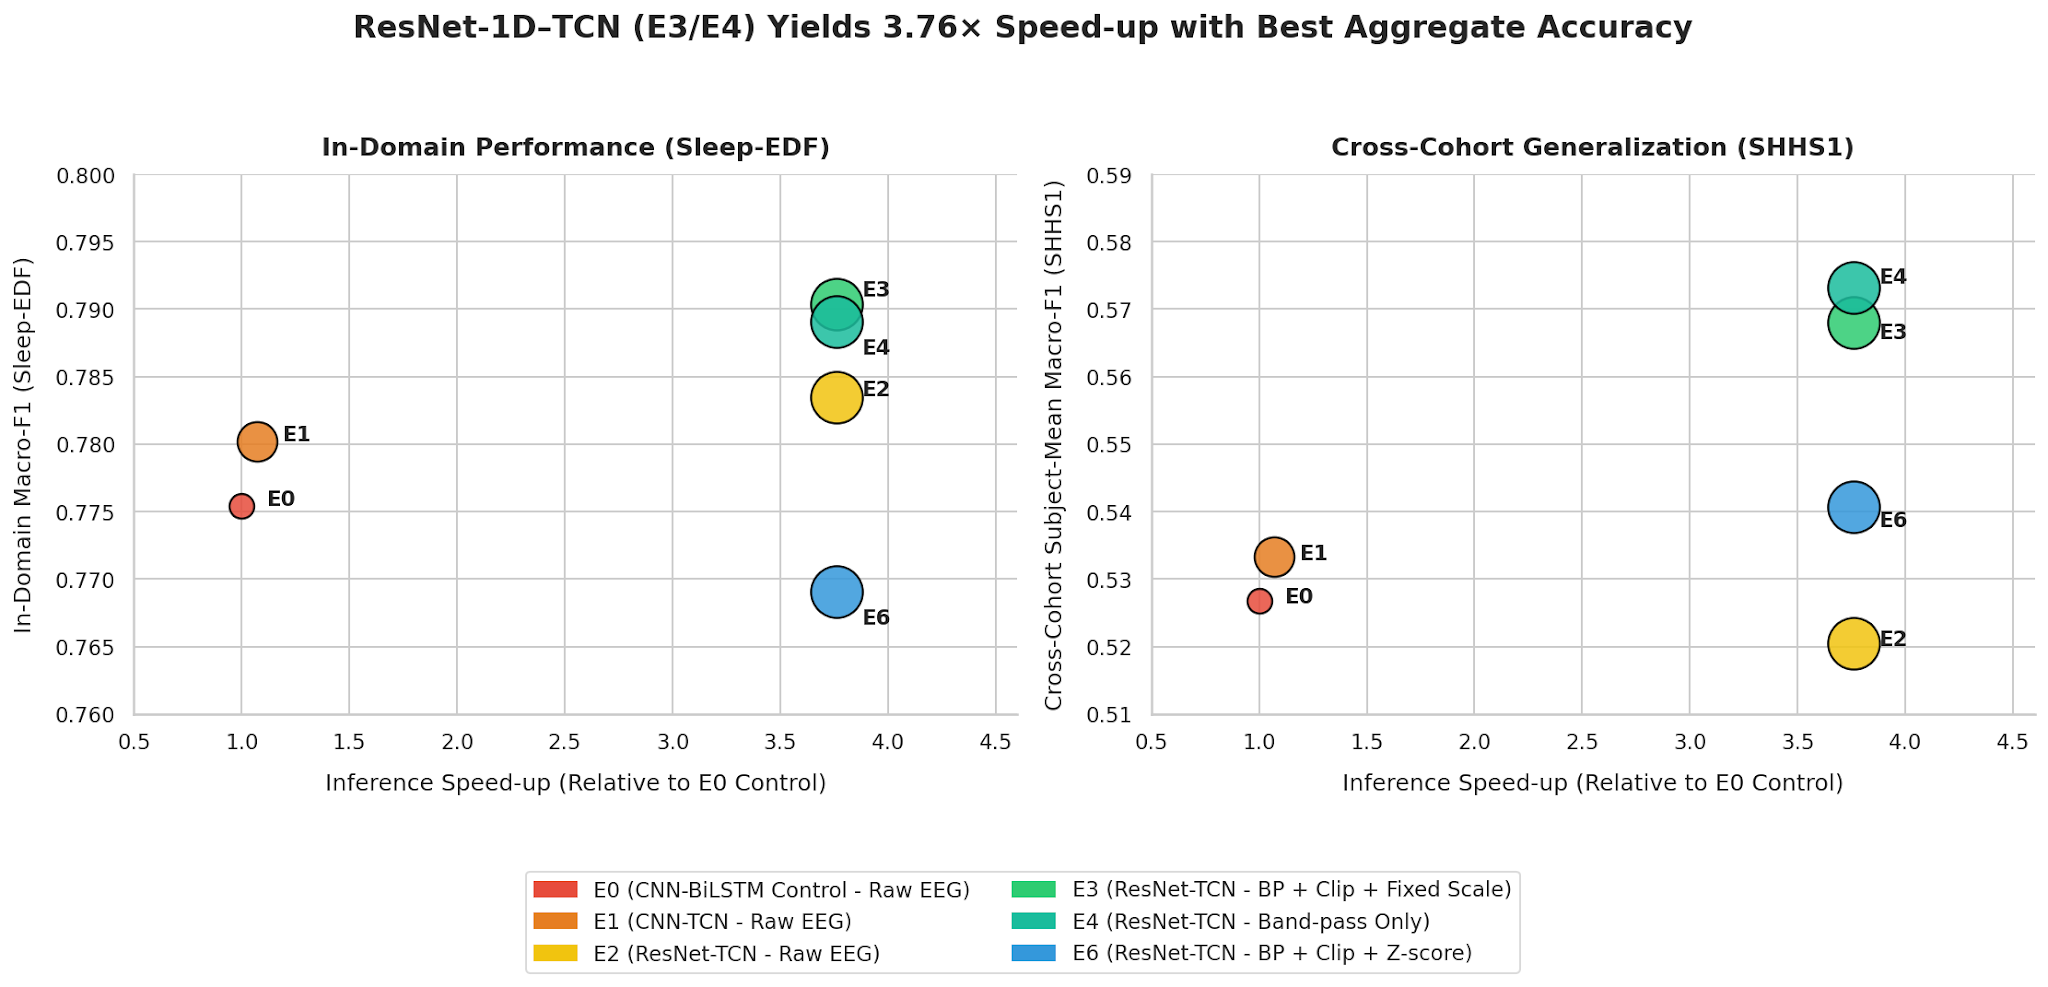
\includegraphics[width=0.85\textwidth]{./figures/gate8_speedup_f1_tradeoff_en.png}
    \caption{\textbf{Inference speed-up versus \mf\ trade-off across Sleep-EDF (in-domain) and SHHS1
    (cross-cohort) datasets.} The proposed ResNet-1D--TCN configuration (E3) achieves a $3.76\times$
    forward-pass speed-up over the CNN--BiLSTM control (E0) while simultaneously improving aggregate
    classification performance in both evaluation settings.}
    \label{fig:speedup_tradeoff}
\end{figure}

\FloatBarrier

In the sequential seed-123 campaign, complete training and validation for E2 and E3 was observed to be
12.2$\times$ and 10.2$\times$ faster than E0. E1 reused E0 encoder checkpoints and therefore has no
end-to-end runtime comparison. Full timings for the specified training and early-stopping recipes are
reported in Supplementary Table~\ref{SM-tab:sup_seed123_runtime}.

\begin{suppfig}[htbp]
    \centering
    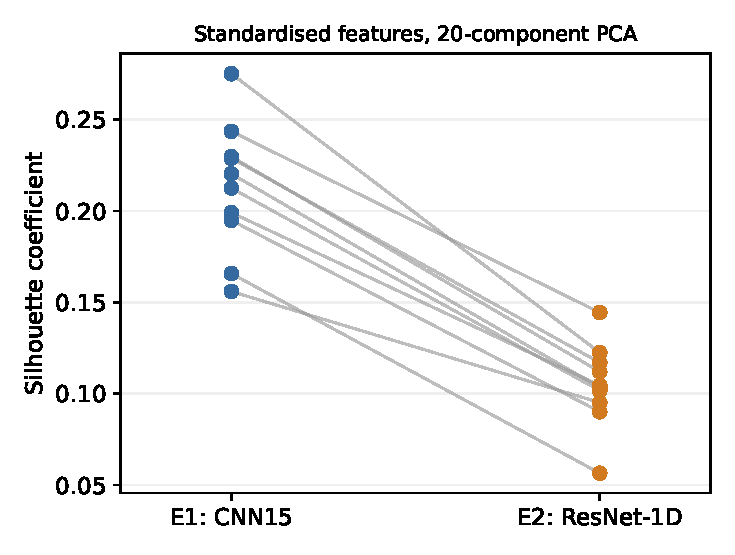
\includegraphics[width=0.75\textwidth]{./figures/gate8_feature_silhouette_en.pdf}
    \caption{\textbf{Silhouette coefficient of standardised features across 20-component PCA.} 
    The figure provides a visual comparison of the spatial representation structure between configuration E1 (15-branch CNN) and E2 (ResNet-1D). Although the ResNet-1D encoder (E2) exhibits lower cluster density (lower Silhouette coefficient) in the PCA-reduced feature space, its single-branch, current-epoch architecture drastically reduces complexity and optimises computational speed when coupled with the TCN sequence model (as quantified in Table~\ref{tab:complexity}). This illustrates the trade-off between feature geometry compactness and end-to-end pipeline efficiency.}
    \label{fig:main_representation_context}
\end{suppfig}

\FloatBarrier

Additional descriptive representation and context-group analyses are reported in
Supplementary Fig.~\ref{SM-fig:sup_representation_context} and Table~\ref{SM-tab:sup_context};
they provide complementary evidence on feature geometry and temporal context.

\subsection{Cross-cohort evaluation on SHHS1}
\label{sec:shhs}

\begin{table}[t]
\centering
\caption{Cross-cohort performance on 180 locked SHHS1 participants (seed 42). All model weights were
trained on Sleep-EDF. E6 additionally uses complete-record, unlabelled target statistics.
Intervals are subject-cluster bootstrap intervals for subject-mean \mf.}
\label{tab:shhs-performance}
\small
\begin{tabular}{lrrrr}
\toprule
\textbf{ID} & \textbf{Subject-mean \mf\ (\ci)} & \textbf{Pooled \mf} & \textbf{Accuracy} & \textbf{$\kappa$} \\
\midrule
E0 & 0.5268 \ $[0.5101, 0.5431]$ & 0.5761 & 0.6648 & 0.5339 \\
E3 & \textbf{0.5680} \ $\boldsymbol{[0.5503, 0.5850]}$ & \textbf{0.6099} & \textbf{0.7016} & \textbf{0.5801} \\
E6 & 0.5407 \ $[0.5227, 0.5584]$ & 0.5732 & 0.6742 & 0.5408 \\
\bottomrule
\end{tabular}
\end{table}

The seed-123 campaign preserves the direction and Holm significance of both SHHS contrasts,
whereas the in-domain E3\,--\,E6 comparison no longer reaches the Holm threshold. This sensitivity result
uses the same SHHS sample; its four-comparison extension family is reported separately in the supplement.

\begin{table}[t]
\centering
\caption{Locked paired comparisons on SHHS1 subject-mean \mf\ ($n = 180$).}
\label{tab:shhs-paired}
\small
\resizebox{\textwidth}{!}{%
\begin{tabular}{llrrrrr}
\toprule
\textbf{Comparison} & \textbf{Role} & $\boldsymbol{\Delta}$ & \textbf{\ci} & $\boldsymbol{p_{\mathrm{Holm}}}$ & \textbf{W/T/L} & $\boldsymbol{\dsign}$ \\
\midrule
E3\,--\,E0 & locked primary & 0.0412 & $[0.0314, 0.0512]$ & $2.65\times10^{-13}$ & 138/0/42 & $+0.533$ \\
E3\,--\,E6 & locked primary & 0.0274 & $[0.0182, 0.0370]$ & $1.87\times10^{-8}$ & 125/0/55 & $+0.389$ \\
\bottomrule
\end{tabular}}
\end{table}

Both locked comparisons support E3 (Table~\ref{tab:shhs-paired}), with improvements in 138 and 125 of
180 subjects, respectively. Sign dominance is $+0.533$ and $+0.389$; the unadjusted exact sign tests
give $p = 3.8\times10^{-13}$ and $1.9\times10^{-7}$. Supporting metrics move
together: relative to E0, E3 gains $0.0338$ pooled \mf, $0.0368$ accuracy and $0.0461$ $\kappa$. Within
$\pm1$ epoch of a transition, E3 gains $0.0366$ over E0 and $0.0183$ over E6.

The secondary configuration analysis gives a different picture. E1\,--\,E0 remains positive but small
($+0.0065$ subject-mean \mf). E2\,--\,E1 is \emph{negative} out of domain
($-0.0128$, interval entirely below zero),
so the bundled replacement of E1's 75-dimensional C/P/N package by the current-epoch 128-dimensional
ResNet-1D representation does not generalise better on unprocessed SHHS signals. Because the entire
feature/context package changes, the reversal cannot be attributed to the encoder alone. The
post-hoc E3\,--\,E2 contrast is the largest observed
configuration difference ($+0.0475$, \ci\ $[0.0372,0.0579]$, $\dsign = +0.633$, 147/180 subjects
improved). E3 and E2 use the same model and specified training recipe with different preprocessing.
This observed contrast is larger than either the sequence-model/recipe or encoder/context contrast
on this sample.

A seed-123 extension evaluating E4 (band-pass only) provides a more specific secondary contrast. E4
reached subject-mean \mf\ $0.5732$, pooled \mf\ $0.6147$, accuracy $0.7064$, $\kappa = 0.5869$ and N1
F1 $0.3492$, exceeding same-seed E2 by $0.0323$ and E3 by $0.0098$. The SHHS-specific preprocessing
audit recorded zero clipped samples across the 200 processed adaptation, validation and test recordings.
E4 and E3 therefore differ on these inputs by the fixed division by 100.
The extension therefore associates band-pass filtering with most of the E4--E2 gain and provides no
evidence that the additional fixed scaling improves transfer. These comparisons remain secondary
because they were conducted after the SHHS sample had been opened.

\FloatBarrier
\subsection{Cross-model errors and their temporal distribution}
\label{sec:gap}

E3's pooled \mf\ is $0.7904$ on Sleep-EDF and $0.6099$ on SHHS1, a difference of $0.1805$.
Because Sleep-EDF uses out-of-fold predictions whereas SHHS uses ten-model ensembles, the $0.1805$
difference is interpreted descriptively. We examine it by class and confusion channel to
determine which errors remain despite E3's aggregate transfer advantage. Throughout this analysis,
A$\rightarrow$B denotes a reference-labelled A epoch predicted as B; it does not denote a physiological
stage transition over time.

N3 is the dominant class loss: E3 N3 F1 falls from 0.8085 on Sleep-EDF to 0.4055 on SHHS1, with
precision 0.9440 but recall 0.2582. E0 shows nearly the same recall (0.2610) and N3$\rightarrow$N2
rate (72.3\% versus 73.1\% for E3), revealing a shared cross-cohort N3 under-detection pattern across
both model families despite E3's aggregate transfer advantage (Table~\ref{tab:cross-model-n3}).
N2$\rightarrow$REM is the second-largest E3 confusion channel.

\begin{table}[t]
\centering\small
\caption{N3 under-detection across the primary SHHS1 configurations (seed 42). All models share
22{,}806 reference N3 epochs. The final column is the proportion of those epochs predicted as N2.}
\label{tab:cross-model-n3}
\begin{tabular}{lrrrrr}
\toprule
\textbf{ID} & \textbf{N3 precision} & \textbf{N3 recall} & \textbf{N3 F1} & \textbf{N3$\to$N2 count} & \textbf{Rate} \\
\midrule
E0 & 0.9007 & 0.2610 & 0.4048 & 16{,}480 & 72.3\% \\
E3 & 0.9440 & 0.2582 & 0.4055 & 16{,}674 & 73.1\% \\
E6 & 0.9052 & 0.2005 & 0.3283 & 17{,}764 & 77.9\% \\
\bottomrule
\end{tabular}
\end{table}

An oracle calculation moves the counts in one selected off-diagonal cell of E3's SHHS confusion
matrix to the correct diagonal cell, then recomputes \mf. Correcting N3$\rightarrow$N2 raises \mf\
to 0.7444; correcting N2$\rightarrow$REM raises it to 0.6596. These changes correspond to 74.5\% and
27.5\% of the observed pooled-score difference. The calculation uses true labels, and its nonlinear
effects are neither additive nor achievable-performance estimates.

The reference-label boundary diagnostic adds temporal detail. For E0 and E3, N3 recall near changes
is 0.6121/0.6326 on Sleep-EDF but only 0.0633/0.0733 on SHHS1. Stable-region SHHS recall remains low
at 0.4008/0.3900. Thus, N3 under-detection extends beyond the boundary neighbourhoods; it cannot be
described solely as an error at label changes. The region definitions and supports are provided in
the supplement, including the epochs omitted from the near-versus-stable comparison.

Furthermore, as detailed in the context ablation study (Figure \ref{fig:context_ablation}), removing the explicit Current/\allowbreak Previous/\allowbreak Next (C/P/N) epoch context does not significantly degrade boundary performance (Holm $p = 1.000$). This strongly supports the premise that sequence models with extended receptive fields, such as the evaluated TCN (253 epochs), successfully capture broad temporal dynamics natively, rendering the localized C/P/N clustering redundant.
\begin{figure}[htbp]
    \centering
    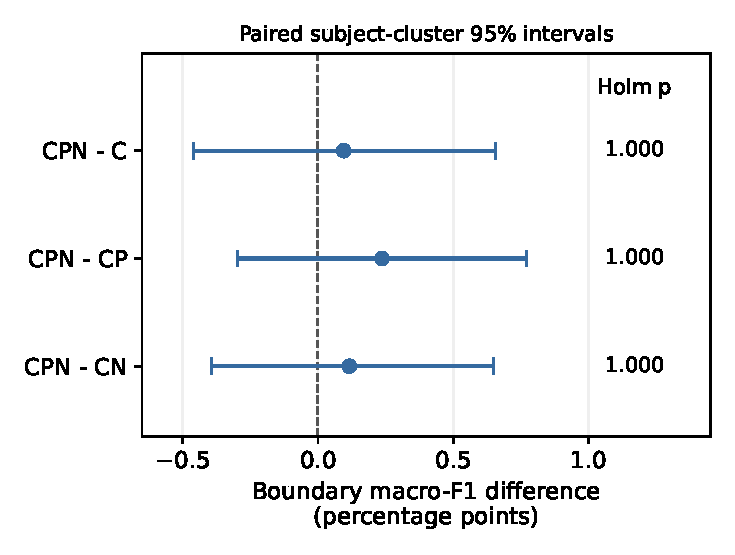
\includegraphics[width=0.75\textwidth]{figures/gate8_context_ablation_effects_en.pdf}
    \caption{\textbf{Context-ablation effects on boundary macro-F1.}}
    \label{fig:context_ablation}
\end{figure}

E6 provides a label-free but transductive sensitivity check. Its complete-target-record $z$-score lowers
N3 recall to 0.2005; boundary-neighbourhood recall is 0.0721 versus 0.0733 for E3.
The tested record-wise normalisation pipeline therefore does not remedy N3 under-detection. Detailed
class-wise, confusion, oracle and transition results are in Supplementary
Tables~\ref{SM-tab:sup_perclass_transfer}--\ref{SM-tab:sup_boundary}.


%==============================================================================
\section{Discussion}

\subsection{What the pipeline comparisons establish}

The main result combines operational and cross-cohort gains at the pipeline level. ResNet-1D--TCN
processes the benchmark input $3.76\times$ faster than the CNN--BiLSTM control,
while using more parameters and memory. Its observed training-and-validation time is also shorter,
although the recipes and stopping rules differ. On the locked SHHS1 sample, E3 improves subject-mean
\mf\ over E0 by 0.0412, with a positive interval and gains in 138 of 180 participants. These results
make the configuration a useful computational alternative with a demonstrated aggregate transfer
benefit in this setting.

The intermediate comparisons explain why that benefit should not be credited simply to a newer
encoder or sequence model. E1--E0 changes both the sequence model and its training recipe;
E2--E1 changes the encoder, feature context and encoder training. Neither contrast reaches the
subject-level Holm threshold on Sleep-EDF, and E2--E1 reverses direction on SHHS1. By contrast,
the observed post-hoc E3--E2 preprocessing difference is larger on SHHS1. The seed-123 extension
further shows that E4, which retains band-pass filtering without fixed scaling, outperforms both E2
and E3 on that sample. Signal handling is therefore a material part of the evaluated model's transfer
behaviour, rather than a negligible implementation detail. These configuration-level comparisons do
not isolate the contribution of each preprocessing operation.

\subsection{Aggregate improvement reveals a shared cross-cohort N3 under-detection pattern}

The class-wise analysis reveals a shared failure mode alongside E3's overall advantage. E0 and E3 both
misclassify more than 72\% of true N3 as N2, with recall near 0.26 despite precision above 0.90.
The alternative E6 pipeline has still lower N3 recall. This common failure persists despite the better
aggregate score. The oracle calculation shows the numerical importance of
N3$\rightarrow$N2 for E3, while the regional analysis shows that the deficit is present in stable
N3 as well as around reference-label changes. Together, these observations identify a more specific
cross-model failure mode for subsequent validation than the overall transfer score alone.

Several explanations remain plausible. The datasets use different EEG derivations, and population,
acquisition and scoring conditions change at the same time. Evidence on slow-wave spatial structure
and N3 scoring criteria provides reasons to investigate these factors~\cite{massimini2004travelling,davidson2025n3},
but the present comparison cannot separate them. Nor does E6 settle the role of amplitude:
record-wise $z$-scoring changes the representation used during source training as well as target
inference. Its failure to remedy N3 under-detection does not rule out amplitude- or montage-related
contributors.

The class-prior difference suggests another testable explanation. Under the assumptions required for
prior correction, its direction would increase N3 and decrease N1 emissions; whether that improves
classification remains to be measured. The observed prediction-to-reference ratios are marginal
counts, not evidence of probability calibration. Calibration, limited fine-tuning and montage-aware
representations are possible follow-ups, not remedies validated by this study. Any intervention should
report N3 precision or false-positive rate alongside recall, because increasing N3 predictions alone
can trade one error for another. N2$\rightarrow$REM is a second candidate channel for E3.

\subsection{Positioning and limits of generalisation}

This study connects paired pipeline comparisons with computational trade-offs and cross-cohort error
structure, complementing work on preprocessing, input representations and conventional/deep pipeline
comparisons~\cite{haghayegh2023sleepinceptionnet,vdd2023traditional}. E0 is a reimplementation of the
ZleepAnlystNet design under the stated protocol, and no target-domain weight update is evaluated; the
results therefore concern locked pipeline transfer rather than adaptation.

The evidence covers one transfer direction and one locked SHHS1 sample. Published scores require matched
subsets, splits, derivations and preprocessing for direct comparison, while the Sleep-EDF out-of-fold and
SHHS ensemble procedures make the cross-cohort score difference descriptive. Two seeds provide a
sensitivity check, and the opened-sample extensions and reference-label diagnostics refine rather than
independently confirm the primary results. These offline evaluations use future context and reference
labels for some diagnostics, so the speed-up and error localisation are not real-time or clinical
validation. Independent validation of the cross-model N3 pattern and a separately specified correction
study remain appropriate next steps.

%==============================================================================
\section{Conclusion}

A shared subject-wise protocol allowed six active configurations to be compared on the same Sleep-EDF
folds; a seventh planned configuration, E5, was excluded before performance analysis because it was
bitwise identical to E4.
The sequence-model/recipe and encoder/context replacements did not establish a stable subject-level
predictive advantage on Sleep-EDF after correction for multiple comparisons. ResNet-1D--TCN offers an operational alternative that is
$3.76\times$ faster in the controlled forward benchmark and 10.2--12.2$\times$ faster in observed
training-and-validation wall-clock time, at the cost of more parameters and memory.

On SHHS1, the fixed-scale E3 procedure outperformed both locked references, while the largest observed
configuration difference was associated with preprocessing under a fixed architecture and training recipe.
These findings demonstrate the value of evaluating signal handling alongside model design, rather than
assuming that an in-domain model ranking will carry over to another cohort.

The class-wise results revealed a shared cross-cohort N3 under-detection pattern across both model
families: E0 and E3 systematically under-call N3 as N2, while E3 also frequently over-calls N2 as REM.
Per-record $z$-scoring does not repair this cross-model failure mode, which appears both near reference-label
changes and within stable SHHS1 regions. The study therefore combines a faster pipeline with improved
aggregate cross-cohort performance and a specific N3 pattern requiring independent validation; whether
calibration, adaptation or montage-aware signal representations can correct it remains an experimental
question.

%------------------------------------------------------------------------------
\subsection*{Reproducibility and data availability}

Code, protocol snapshots, data partitions and aggregate analyses are retained in the project repository
at \url{https://github.com/quanuiter/SleepTCN}. The repository does not contain restricted participant-
level SHHS data, identifiers or predictions.
Sleep-EDF Expanded is available through PhysioNet; SHHS access is managed by NSRR. Participant-level
SHHS records and predictions are not included in the manuscript package. The historical snapshot
\texttt{configs/shhs\_zero\_shot\_v1.json} matches the protocol hash in the original SHHS run manifest.
The primary campaign's 540 ensemble prediction files were checked against their recorded SHA-256 values,
and their confusion counts reproduce the reported pooled results. This verifies those retained artifacts;
it is not a regeneration of predictions or an end-to-end rerun. The expanded post-run protocol record
is preserved separately. Further provenance details are given in the supplement and the repository
artifact index.

The experimental revision is fixed at Git commit
\href{https://github.com/quanuiter/SleepTCN/commit/f7c22e76022b8e24ac8d1343a39a990d42a1b3e2}{\texttt{f7c22e7}}.

\subsection*{Ethics}

This study is a secondary analysis of de-identified repository data; no new participants were recruited.
The authors confirm that access to SHHS for this analysis was obtained through the National Sleep
Research Resource and that no ethics approval was required for this secondary analysis of de-identified
repository data. No new participants were recruited and no approval number is asserted.

\subsection*{Funding}

This work received approximately VND 6,000,000 in student support from the University of Information
Technology, Vietnam National University Ho Chi Minh City.
The underlying Sleep Heart Health Study was supported by National Heart, Lung, and Blood Institute
cooperative agreements U01HL53916, U01HL53931, U01HL53934, U01HL53937, U01HL64360, U01HL53938,
U01HL53940, U01HL53941 and U01HL63463.

\subsection*{Acknowledgements}
This research was supported by The VNUHCM University of Information Technology’s Scientific
Research Support Fund.

\subsection*{CRediT authorship contribution statement}

Ngo Nhat Quan: Conceptualization, Methodology, Software, Data curation, Formal analysis,
Investigation, Visualization, Writing -- original draft, Writing -- review and editing. Pham Thai Son:
Validation, Investigation, Visualization, Writing -- review and editing.

\subsection*{Declaration of competing interests}

The authors declare no competing interests.

\subsection*{Declaration of generative AI and AI-assisted technologies}

OpenAI Codex assisted with English-language editing, manuscript organisation, consistency checks
against code and archived results, and reproducible plotting of existing aggregate data. It did not
generate new experimental observations or replace the archived predictions. No other AI tool was used
for this manuscript preparation. Both authors have read and approved the final manuscript and this
disclosure; the authors remain responsible for the submitted content.

%------------------------------------------------------------------------------
\begingroup
\small
\bibliographystyle{ieeetr}
\bibliography{references}
\endgroup

\end{document}
